\newpage
\subsubsection{Basic Fish}
\label{X-Wing}
Die Techniken \textit{X-Wing}, \textit{Swordfish} und \textit{Jellyfish} sind die einfachsten Unterarten der Fische. Sie funktionieren nach dem selben Prinzip, nur dass eine unterschiedliche Anzahl an Figuren betrachtet wird, ähnlich zu \textit{Naked Subset} und \textit{Hidden Subset}. Hier wird stellvertretend die Technik \textit{X-Wing} erklärt und am Beispiel gezeigt.\\
Dazu sucht man zwei Spalten oder Zeilen, die ausschließlich in den selben zwei Zellen einen bestimmten Kandidaten, die Fischziffer, beinhalten. Nun kann man aus dem jeweils anderen Paar von Figuren (Spalte oder Zeile), deren Position durch die zwei gefundenen Zellen festgelegt wird, alle Fischziffern löschen, die nicht gleichzeitig in einer der zuerst ausgesuchten Figuren liegen.\\
Da die Fischziffer in den beiden zuert ausgesuchten Figuren nur an jeweils zwei Stellen liegen kann und diese sich paarweise gegeinseitig ausschließen ist klar, dass jedes Vorkommen der Fischziffer in den zuletzt ausgesuchten Figuren in der Überschneidung mit den ersten Figuren liegen muss.

\begin{figure}[h]
\begin{center}
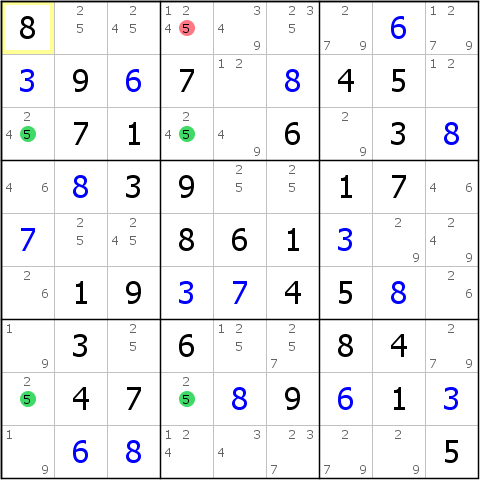
\includegraphics{./img/x_wing.png}
\caption{Basic Fish - X-Wing}
\end{center}
\end{figure}

Ein Beispiel für die Technik \textit{X-Wing} findet sich in \textbf{Abbildung 2.10}. Hier wählen wir zuerst die Figuren Zeile 3 und 8. Diese enthalten die Fischziffer 5 nur an den Stellen 1 und 4. Wichtig ist, dass es in den beiden Zeilen die gleichen Positionen sind. Wir betrachten nun zwei Fälle. Steht in z3s4 die Ziffer 5, dann kann man die rot markierte Ziffer sofort löschen. In Fall zwei steht die Ziffer 5 in z3s1. Daher kann sie nicht in z8s1 stehen und müsste daher in z8s4 eingesetzt werden. Das würde ebenfalls die rot markierte Ziffer ausschließen. Da sie in beiden möglichen Fällen nicht in z1s4 stehen kann, kann sie gelöscht werden.